\chapter{Parameter Estimation: Bayes' Box}
One of the most important ways of using Bayes' rule is in the topic
called {\it parameter estimation}. Parameter estimation is a fairly common
situation in statistics. In fact, it is possible to interpret almost any
problem in statistics as a parameter estimation problem and approach it
in this way!

Firstly, what is a parameter? Well, it is just a fancy term for a quantity or
a number that is unknown. For example, how many people are currently in New
Zealand? Well, a Google search suggests 4.405 million. But that does not mean
there are {\bf exactly} 4,405,000 people. It could be a bit more or a bit
less. Maybe it is 4,405,323, or maybe it is 4,403,886. We don't really know.
We could call the true number of people in New Zealand right now $\theta$, or
we could use some other letter or symbol if we liked.

The key is to realise that we can use the Bayes Box like in previous chapters,
but now, our list of possible hypotheses is a list of possible values for
the unknown parameter. For example, a Bayes Box for the precise number of
people in New Zealand might look something like this:
\begin{table}[h!]
\begin{center}
\begin{tabular}{|c|c|c|c|c|}
\hline
{\bf Possible Hypotheses} & {\tt prior} & {\tt likelihood} &
{\tt prior $\times$ likelihood} & {\tt posterior}\\
\hline
\ldots & \ldots & \ldots & \ldots & \ldots\\
$\theta = 4404999$ & 0.000001 & \ldots   & \ldots  & \ldots\\
$\theta = 4405000$ & 0.000001 & \ldots   & \ldots  & \ldots\\
$\theta = 4405001$ & 0.000001 & \ldots   & \ldots  & \ldots\\
$\theta = 4405002$ & 0.000001 & \ldots   & \ldots  & \ldots\\
$\theta = 4405003$ & 0.000001 & \ldots   & \ldots  & \ldots\\
$\theta = 4405004$ & 0.000001 & \ldots   & \ldots  & \ldots\\
$\theta = 4405005$ & 0.000001 & \ldots   & \ldots  & \ldots\\
$\theta = 4405006$ & 0.000001 & \ldots   & \ldots  & \ldots\\
\ldots & \ldots & \ldots & \ldots & \ldots\\
\hline
Totals: & 1 & & \ldots & 1\\
\hline
\end{tabular}
\end{center}
\end{table}

There are a few things to note about this Bayes' box. Firstly, it is big, which
is why I just put a bunch of ``\ldots''s in there instead of making up numbers.
There are lots of possible hypotheses, each one corresponding to a possible value
for
$\theta$. The prior probabilities I have put in the 2nd column were for
illustration purposes, they needn't necessarily all be the same. But all the
stuff we've seen in smaller examples still applies here. The likelihoods will
still be calculated by seeing how the probability of the data depends on the
value of the unknown parameter. You still go through all the same steps,
multiplying prior times likelihood and then normalising that to get the
posterior probabilities for all of the possibilities listed. Note that a set
of possible values together with the probabilities is what is commonly termed
a {\it probability distribution}. In basic Bayesian problems, like in the
introductory chapters, we start with some prior probabilities and update them
to get posterior probabilities. In parameter estimation, we start with a prior
{\it distribution} for the unknown parameter(s) and update that to get a
posterior distribution for the unknown parameter(s).

\begin{framed}
{\bf
A quantity which has a probability associated with each possible value is
traditionally called a ``random variable''. Random variables have probability
distributions associated with them. In Bayesian stats, an unknown
parameter looks mathematically like a ``random variable'', but nothing is
varying or fluctuating. We put a probability distribution there to describe our
uncertainty about what the true value is.}
\end{framed} 

\section{Parameter Estimation: Bus Example}
This is a beginning example of parameter estimation from a Bayesian point of
view. It shows the various features that are always present in a Bayesian
parameter estimation problem: there will be a prior distribution, the likelihood,
and the posterior distribution.

After moving to Auckland, I decided that I would take the bus to work
each day. However, I wasn't very confident with the bus system, so for the first
week I just took the first bus that came along and was heading in the right
direction (towards the city). In the first week, I caught 5 morning buses.
Of these 5 buses, two of them took me to the right place, while three of them
took me far from work, leaving me with an extra 20 minute walk. Given this
information, what can we say about the value of $\theta$, the proportion of the
buses that are actually the correct bus?

In principle, $\theta$ could take any real value between 0 and 1.
To begin, we shall make an approximation and assume that the possible values
for $\theta$ can only be one of the following numbers:
\begin{center}
$\{0, 0.1, 0.2, 0.3, 0.4, 0.5, 0.6, 0.7, 0.8, 0.9, 1\}$.
\end{center}
This discrete
approximation means that we can use a Bayes' Box. The first things to fill out
in the Bayes' Box are the possible values and the prior probabilities (the prior
distribution). For starters, let us assume that before we got the data (two
successes out of 5 trials), we were very uncertain about the value of $\theta$,
and this can be modelled by using a uniform prior distribution. There are 11
possible values for $\theta$ that are being considered, so the probability of
each is $1/11 = 0.0909$.

For the likelihood, we need to think about what the 

\begin{table}[ht!]
\begin{center}
\begin{tabular}{|c|c|c|c|c|}
\hline
\tt{possible Values} & \tt{prior} & \tt{likelihood} & \tt{prior} $\times$ \tt{likelihood} & \tt{posterior}\\
$\theta$ & $p(\theta)$ & $p(x|\theta)$ & $p(\theta)p(x|\theta)$ & $p(\theta|x)$\\
\hline
0 & 0.0909 & 0 & 0 & 0\\
0.1 & 0.0909 & 0.0729 & 0.0066 & 0.0437\\
0.2 & 0.0909 & 0.2048 & 0.0186 & 0.1229\\
0.3 & 0.0909 & 0.3087 & 0.0281 & 0.1852\\
0.4 & 0.0909 & 0.3456 & 0.0314 & 0.2074\\
0.5 & 0.0909 & 0.3125 & 0.0284 & 0.1875\\
0.6 & 0.0909 & 0.2304 & 0.0209 & 0.1383\\
0.7 & 0.0909 & 0.1323 & 0.0120 & 0.0794\\
0.8 & 0.0909 & 0.0512 & 0.0047 & 0.0307\\
0.9 & 0.0909 & 0.0081 & 0.0007 & 0.0049\\
1 & 0.0909 & 0 & 0 & 0\\
\hline
Totals & 1 & & 0.7145 & 1\\
\hline
\end{tabular}
\caption{The completed Bayes' Box for the bus problem (binomial likelihood).\label{tab:bus_bayes_box}}
\end{center}
\end{table}

To get the likelihoods, we need to think about what our experiment is doing.
In particular, we should imagine that we knew the value of $\theta$ and were
trying to predict what experimental outcome would occur. If there are $N=5$
repetitions of an experiment and the ``success'' probability is $\theta$ each time,
then the number of ``successes'' $x$ has a binomial distribution:
\begin{eqnarray}
p(x|\theta) &=& \left(\begin{array}{c}N \\ x\end{array}\right)
\theta^x\left(1-\theta\right)^{N - x}.\label{eq:binomial_likelihood2}
\end{eqnarray}
This is the probability mass function for $x$. Since there are five trials
($N=5$), the number of successes $x$ must be one of 0, 1, 2, 3, 4, or 5.
If $\theta$ is a high number close to one, then we would expect the resulting
value of the data $x$ to be something high like 4 or 5. Low values for $x$ would
still be possible but they would have a small probability. If $\theta$ is a
small number, we would expect the data to be 0, 1, or 2, with less probability
for more successes than that. This is just saying in words what is written
precisely in Equation~\ref{eq:binomial_likelihood}. The probability distribution
for the data $x$ is plotted in Figure~\ref{fig:binomial} for three illustrative
values of the parameter $\theta$.
\begin{figure}[h!]
\begin{center}
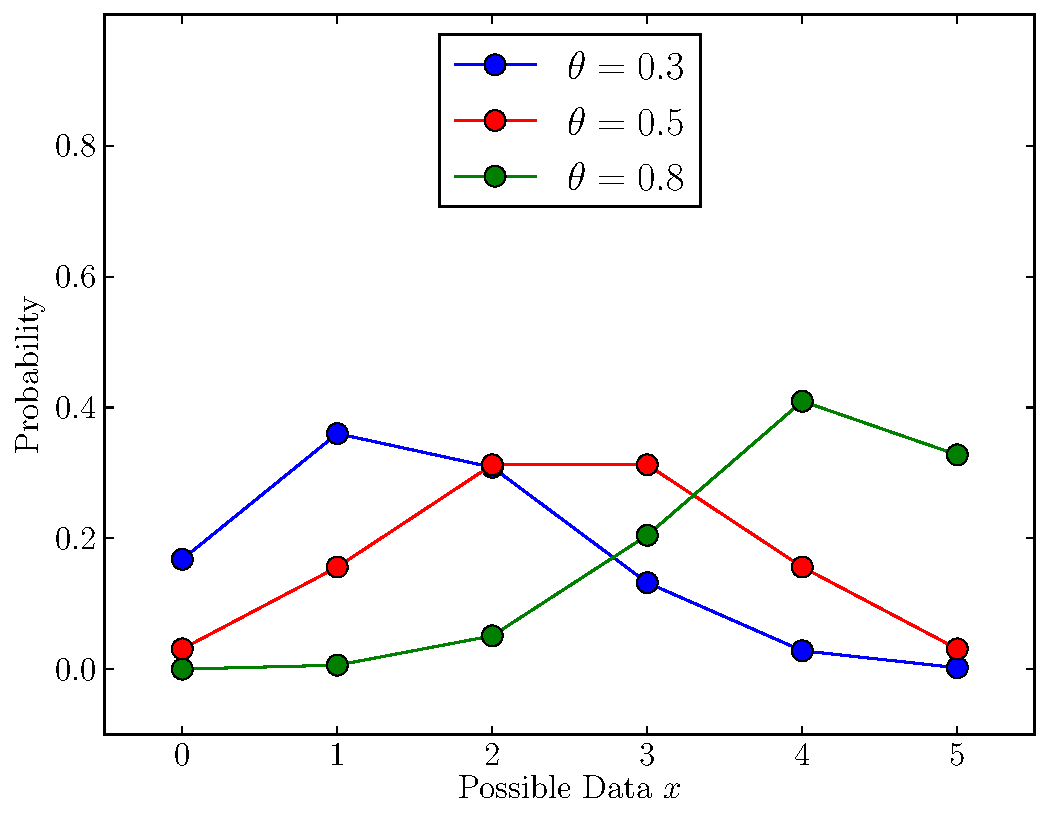
\includegraphics[scale=0.6]{Figures/binomial.pdf}
\caption{The binomial likelihood, viewed as a probability distribution for the
data $x$, for three different values of the parameter $\theta$. If $\theta$ is
low then we would expect to see lower values for the data. If $\theta$ is high
then high values are more probable (but all values from 0 to 5 inclusive are
{\it possible}).
\label{fig:binomial}}
\end{center}
\end{figure}
To obtain the actual likelihood values that go into the Bayes' Box, we can
simply substitute in the known values $N=5$ and $x=2$:
\begin{eqnarray}
P(x=2|\theta) &=& \left(\begin{array}{c}5 \\ 2\end{array}\right)
\theta^2\left(1-\theta\right)^{5 - 2}\\
&=& 10\times\theta^2\left(1-\theta\right)^3.\label{eq:binomial_likelihood3}
\end{eqnarray}
The resulting equation depends on $\theta$ only! We can go through the list of
$\theta$ values and get a numerical answer for the likelihood $P(x=2|\theta)$,
which is what we need for the Bayes' Box. The final steps are, as usual, to multiply the prior by the likelihood and then normalise that to get the posterior distribution.

There are a few interesting values in the likelihood column that should help you
to understand the concept of likelihood a bit better. Look at the likelihood for
$\theta = 0$: it is zero. What does this mean? It means that if we imagine
$\theta=0$ is the true solution, the probability of obtaining the data that we
got ($x=2$ successes) would be zero. That makes sense! If $\theta=0$ that means
that none of the buses are the ``good'' buses -- so how could I have caught a
good bus twice? The probability of that is zero.

The likelihood for $\theta=1$ is also zero for similar reasons. If all of the
buses are good, then having 2/5 successes is impossible -- you would get 5/5
with 100\% certainty. So $P(x=2|\theta=1) = 0$. The likelihood is highest
for $\theta = 0.4$, which just so happens to equal 2/5. This means that this
value for $\theta$ is the one that makes the data the least surprising. It does
not necessarily mean that $\theta=0.4$ is the most probable value, that depends
on the prior as well (but with a uniform prior, it will end up being that way).

\section{Prediction}
We have now seen how to use information (data) to update from a prior distribution
to a posterior distribution when the set of possible values is discrete. The
posterior distribution is the complete answer to the problem: it tells us exactly
how strongly we should believe in the various possible solutions. However, there
are other things we might want to do with this information. Predicting the future
is one! It's fun, but risky. Here we will look at how it is done using the Bayesian
framework, continuing with the bus example. To be concrete, we are interested
in the following question: {\it what is the probability that I will catch the
right bus tomorrow?}. This is like asking a question about what the future data
will be.

Suppose we knew that the true value of $\theta$ was 0.3. Then, we would know that
the probability of catching the right bus tomorrow is 0.3. If we knew that the
true value of $\theta$ was 0.4, we would say that the probability of catching
the right bus tomorrow is 0.4. The problem is, we don't know what the true value
is. We only have the posterior distribution. Luckily, the sum rule of
probability can help us out. We are interested in whether I will get the good
bus tomorrow. There are 11 different ways that can happen: either $\theta=0$ and
I get the good bus, or $\theta=0.1$ and I get the good bus, or $\theta=0.2$ and
I get the good bus, and so on. These 11 ways are all mutually exclusive, that is,
only one of them can be true (since $\theta$ is actually just a single number).
Mathematically, this can be written using the sum rule:
\begin{eqnarray}
P(\textnormal{good bus tomorrow} | x) &=& \sum_{\theta}
p(\theta | x)P(\textnormal{good bus tomorrow} | \theta, x)\\
&=& \sum_{\theta}
p(\theta | x)\theta
\end{eqnarray}
This says that the total probability for a good bus tomorrow (given the data)
is given by going through each possible $\theta$ value, working out the probability
{\it assuming that $\theta$ value is true}, multiplying that by the probability
(given the data) that that $\theta$ value is actually true, and summing. In this
problem, because $P(\textnormal{good bus tomorrow} | \theta, x) = \theta$, it
just so happens that the probability for tomorrow is the expectation value of
$\theta$ using the posterior distribution.

The R code for computing the Bayes' Box in this problem is given below. This is
very much like a lot of the problems we will work on in labs.

\begin{framed}
\begin{verbatim}
# Make a vector of possibilities
theta = seq(0, 1, by=0.1)

# Corresponding vector of prior probabilities
prior = rep(1/11,11)

# Likelihood. Notice use of dbinom() rather than formula
lik = dbinom(2,5,theta)

# Prior times likelihood, then normalise to get posterior
h = prior*lik
post = h/sum(h)

# Probability for good bus tomorrow (prediction!)
prob_tomorrow = sum(theta*post)
\end{verbatim}
\end{framed}


\chapter{Parameter Estimation: Analytical Methods}
Analytical methods are those that can be carried out with a pen and paper,
the ``old school'' way before we all started using computers. There are some
problems in Bayesian statistics that can be solved in this way, and we will
see one or two of them in this course.

Let's look at the {\it binomial likelihood} problem again, with the familiar
bus example. Out of $N=5$ attempts at a ``repeatable'' experiment, there were
$x=2$ successes. From this, we want to infer the value of $\theta$, the
success probability that applied on each trial. Because of its meaning, we know
with 100\% certainty that $\theta$ must be between 0 and 1 (inclusive).

Recall that, if we knew the
value of $\theta$ and wanted to predict the data $x$ (regarding $N$ as being
known in advance), then we would use the binomial distribution:
\begin{eqnarray}
p(x|\theta) &=& \left(\begin{array}{c}N \\ x\end{array}\right)
\theta^x\left(1-\theta\right)^{N - x}.\label{eq:binomial_likelihood}
\end{eqnarray}

Let's use a uniform prior for $\theta$.
The equation for a uniform probability density is:
\begin{eqnarray}
p(\theta) &=& \left\{
\begin{array}{lr}
1, & 0 \leq \theta \leq 1\\
0, & \textnormal{otherwise}
\end{array}
\right.\label{eq:uniform}
\end{eqnarray}
To find the posterior probability density for $\theta$, we use the ``parameter
estimation'' form of Bayes' rule:
\begin{eqnarray}
\textnormal{posterior} \propto \textnormal{prior} \times \textnormal{likelihood}\\
p(\theta|x) \propto p(\theta)p(x|\theta).
\end{eqnarray}
We already wrote down the equations for the prior and the likelihood, so we
just need to multiply them together.
\begin{eqnarray}
p(\theta|x) &\propto& p(\theta)p(x|\theta)\\
&\propto& 1 \times \left(\begin{array}{c}N \\ x\end{array}\right)
\theta^x\left(1-\theta\right)^{N - x}
\end{eqnarray}
as long as $\theta \in [0, 1]$. There is a handy tip you can use a lot of the
time when working things out analytically. Notice that the ``parameter estimation''
form of Bayes' rule has a proportional sign in it, not an equals sign. That's
because the prior times the likelihood can't actually be the posterior
distribution because it may not be normalised -- the sum or integral is not 1.
However, the equation still gives the correct shape of the probability density
function: the way it depends on $\theta$. The reason this is helpful is that
you can save ink: if there are some factors out the front of your expression
that don't involve the parameter (in this case, $\theta$), you can ignore them!
The proportional sign will take care of them. In this case, it means we can
forget about the pesky ``$N$ choose $x$'' term, and just write:
\begin{eqnarray}
p(\theta|x) &\propto& \theta^x\left(1-\theta\right)^{N - x}\\
&\propto& \theta^2\left(1-\theta\right)^3.
\end{eqnarray}
The final step was to substitute in the actual values of $N$ and $x$ instead of
leaving the symbols there. That's it! We have the correct shape of the
posterior distribution. We can use this to plot the posterior, as you can see
in Figure~\ref{fig:bus_inference}.

\begin{figure}[h!]
\begin{center}
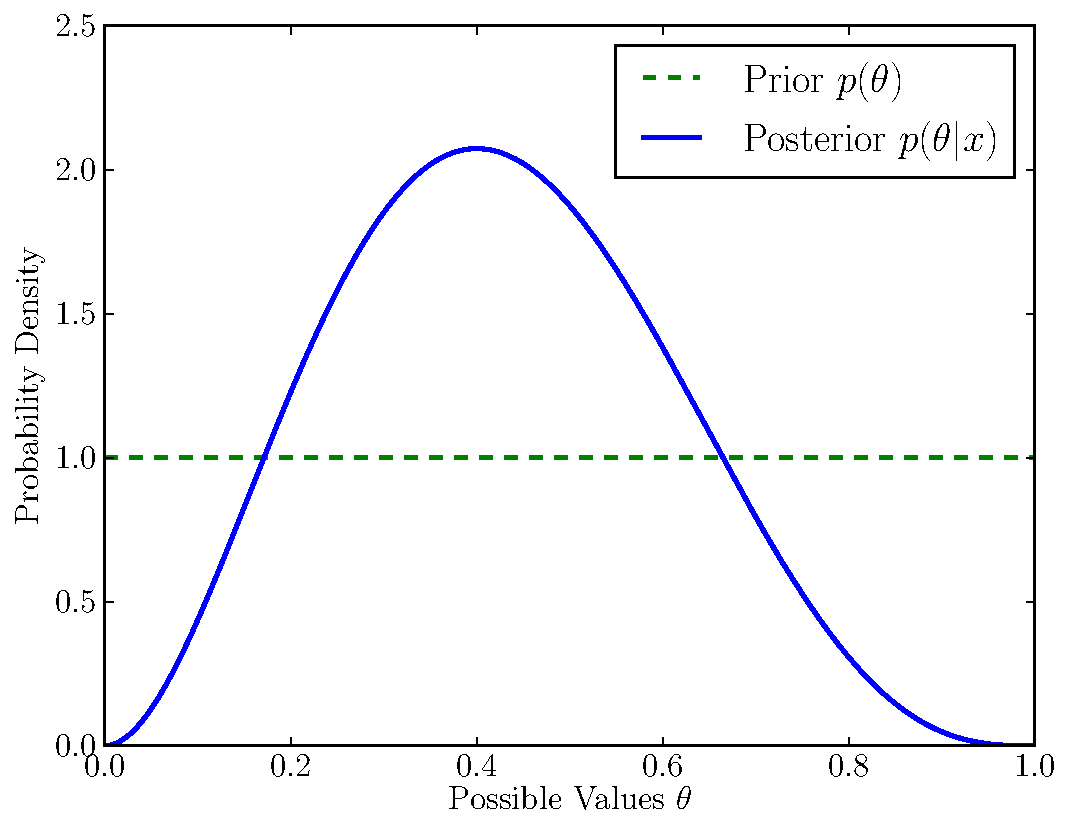
\includegraphics[scale=0.6]{Figures/bus_inference.pdf}
\caption{\label{fig:bus_inference}}
\end{center}
\end{figure}

\section{Statistician's Notation}
While it is very helpful to know the full equations for different kinds of
probability distributions (both discrete ones and continuous ones), if you only
want to say what a distribution is. Instead of saying ``the prior for $\theta$
is uniform between 0 and 1'', or giving the formula for the prior distribution
(Equation~\ref{eq:uniform}), you can write:
\begin{eqnarray}
\theta \sim \textnormal{Uniform}(0, 1)
\end{eqnarray}
or, even more concisely:
\begin{eqnarray}
\theta \sim U(0, 1).
\end{eqnarray}
This notation conserves ink, and is good for quick communication. It is also
very helpful because when we come to use JAGS in later chapters, it likes
things to be written this way.

We can also write the binomial likelihood in this way, instead of writing out
the full equation. We can write:
\begin{eqnarray}
x | \theta \sim \textnormal{Binomial}(N, \theta)
\end{eqnarray}
This says that, if we knew the value of $\theta$, $x$ would have a binomial
distribution with $N$ trials and success probability $\theta$. We can also
make this more concise:
\begin{eqnarray}
x \sim \textnormal{Bin}(N, \theta)
\end{eqnarray}
The differences here are that ``Binomial'' has been shortened to ``Bin'' and
the ``given $\theta$'' part has been left out. However, we see that there is
a $\theta$ is present on the right hand side, so the ``given $\theta$'' must
be understood implicitly.

